\documentclass[11pt]{report}
\usepackage{eso-pic,graphicx}
\usepackage[export]{adjustbox}
\usepackage{url}
\usepackage{amsmath}
\usepackage[top=2cm, bottom=2cm, outer=2cm, inner=2cm]{geometry}
\begin{document}
%\AddToShipoutPictureBG*{
\includegraphics[width=\paperwidth,height=\paperheight]{images/bkgrnd}}
\begin{center}
\vspace*{2cm}
\textsf{\begin{Huge}
\textbf{ELP­718 ­ Telecom Software Laboratory \\
1st Semester, 2016-18 \\
Abhishek Mishra\\
08 Nov 2016, 5pm\\
Assignment-13}\\
\end{Huge}}
\vspace*{6cm}

\includegraphics[scale=0.12, center]{images/iitlogo}
\end{center}
\pagebreak
\tableofcontents
\vspace{5cm}
\pagebreak
\section{Introduction}
\vspace*{1cm}
This assignment aims to provide a better understanding of the following topics:\\
\begin{flushleft}
1. \textbf{Socket Programming}\\
Sockets allow communication between two different processes on the same or different machines. To be more precise, it's a way to talk to other computers using standard Unix file descriptors. In Unix, every I/O action is done by writing or reading a file descriptor. A file descriptor is just an integer associated with an open file and it can be a network connection, a text file, a terminal, or something else.\\
To a programmer, a socket looks and behaves much like a low-level file descriptor. This is because commands such as read() and write() work with sockets in the same way they do with files and pipes.
\end{flushleft}
\newpage
\section{Problem Statement 1}
Write a lex/lex-yacc code to evaluate the consistency of given .pgn file, which record chess moves in given game. You have to find any wrong notations and its location in metadata or using move number\\
%\begin{gather*}
%\textbf{Student}(Stu\_id, Name, Gender);\\
%\textbf{Course}(Course\_id, Course name, Instructor);\\
%\textbf{Enroll}(Stu\_id, Course\_id);\\
%\textbf{Grades}(Stu\_id, Course\_id, Grade);\\
%\end{gather*}
	
\subsection{Assumptions}
The files that are read follow strict pgn rules.
Design Database for given system using MySQL i.e. create one database and the relational tables described above. Also write a python code to populate the tables.\\
The generated table looks like this:\\
\section{Problem Statement 2}
You are given with list of students in given format with their marks in respective subject. You have to calculate their SGPA and write that down after every student. Use Lex and Yacc to for the purpose, such that it will check consistency of input format and calculate CGPA.\\
%\begin{gather*}
%\textbf{Student}(Stu\_id, Name, Gender);\\
%\textbf{Course}(Course\_id, Course name, Instructor);\\
%\textbf{Enroll}(Stu\_id, Course\_id);\\
%\textbf{Grades}(Stu\_id, Course\_id, Grade);\\
%\end{gather*}
	
\subsection{Assumptions}
The files that are read follow strict pgn rules.
Design Database for given system using MySQL i.e. create one database and the relational tables described above. Also write a python code to populate the tables.\\
The generated table looks like this:\\
\section{Structure Chart}
\begin{figure}[h!]
\centering
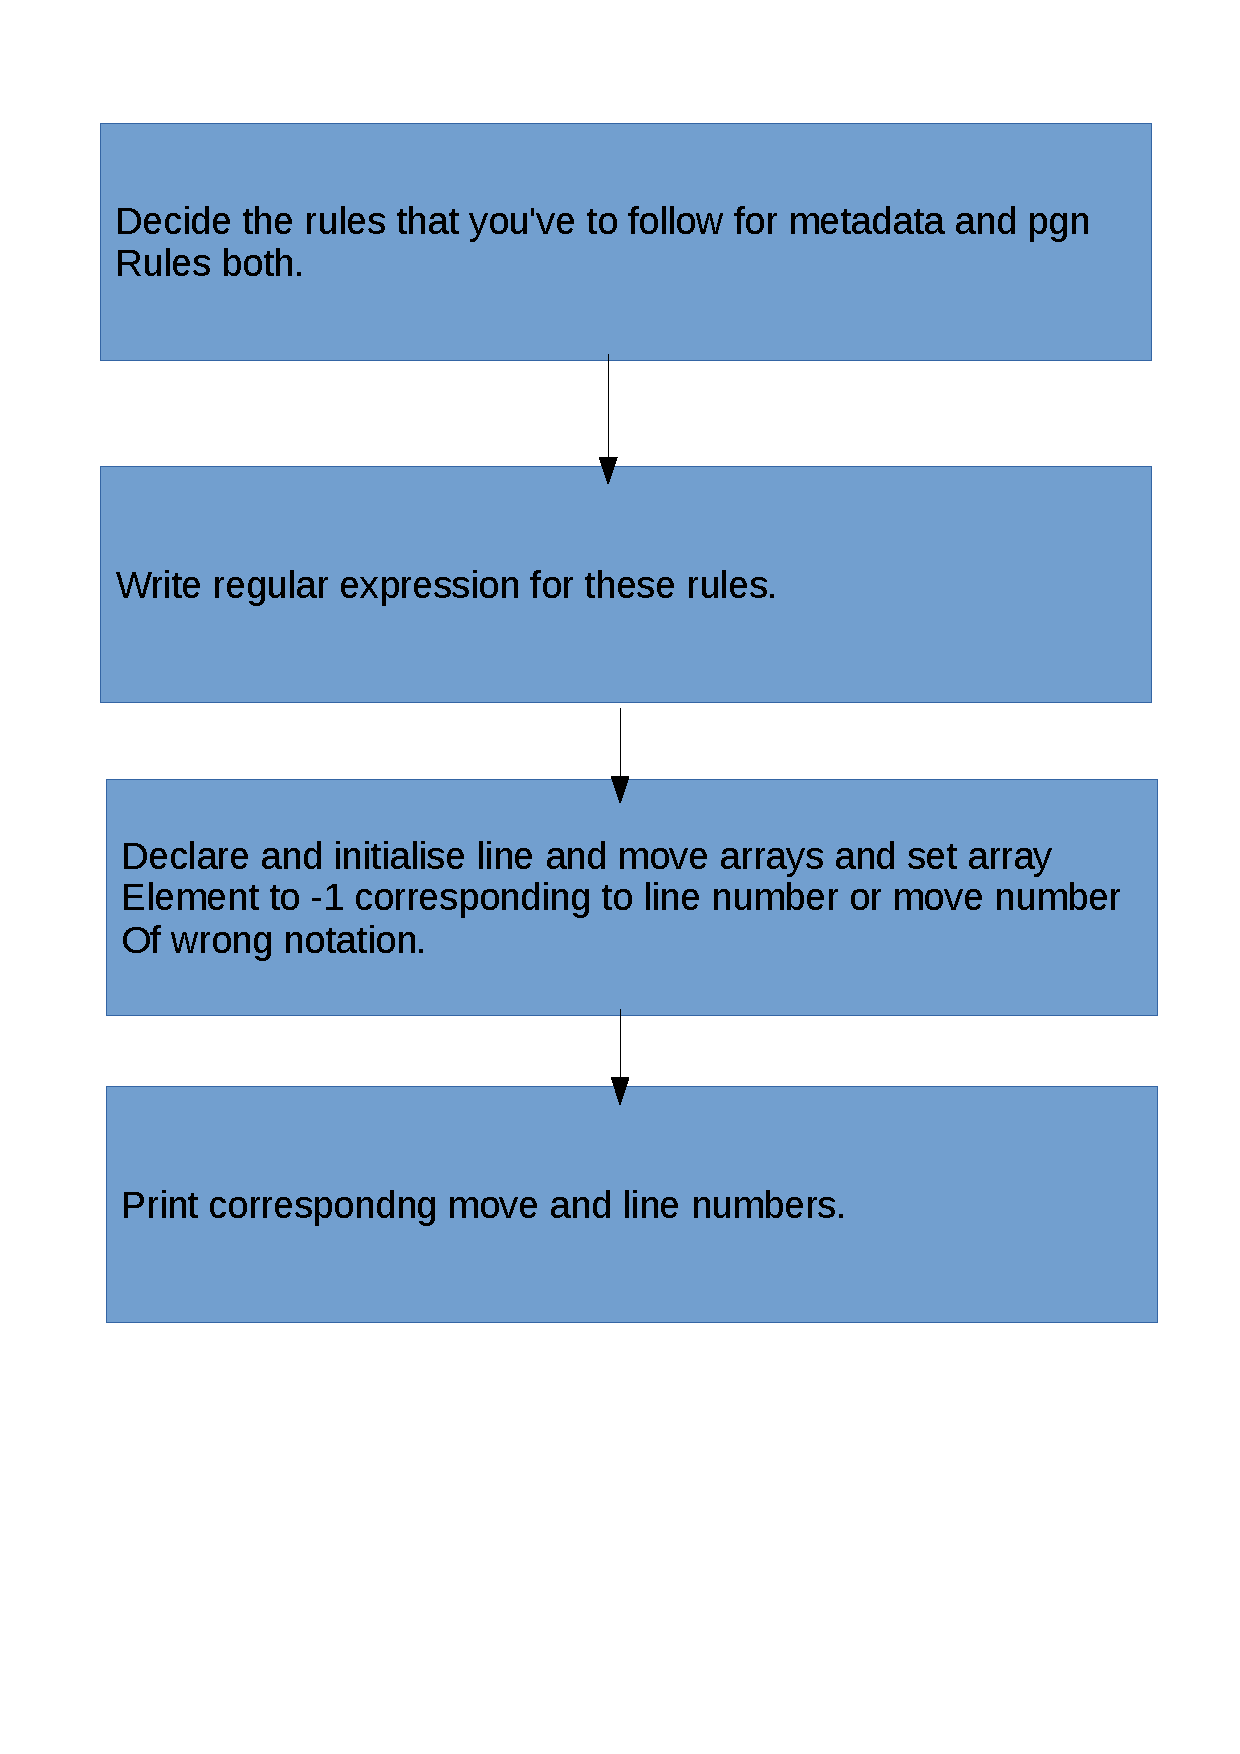
\includegraphics[scale=0.5]{images/sc1}
\caption{Structure chart for Problem 1}	
\end{figure}
\pagebreak
\begin{figure}[h!]
\centering
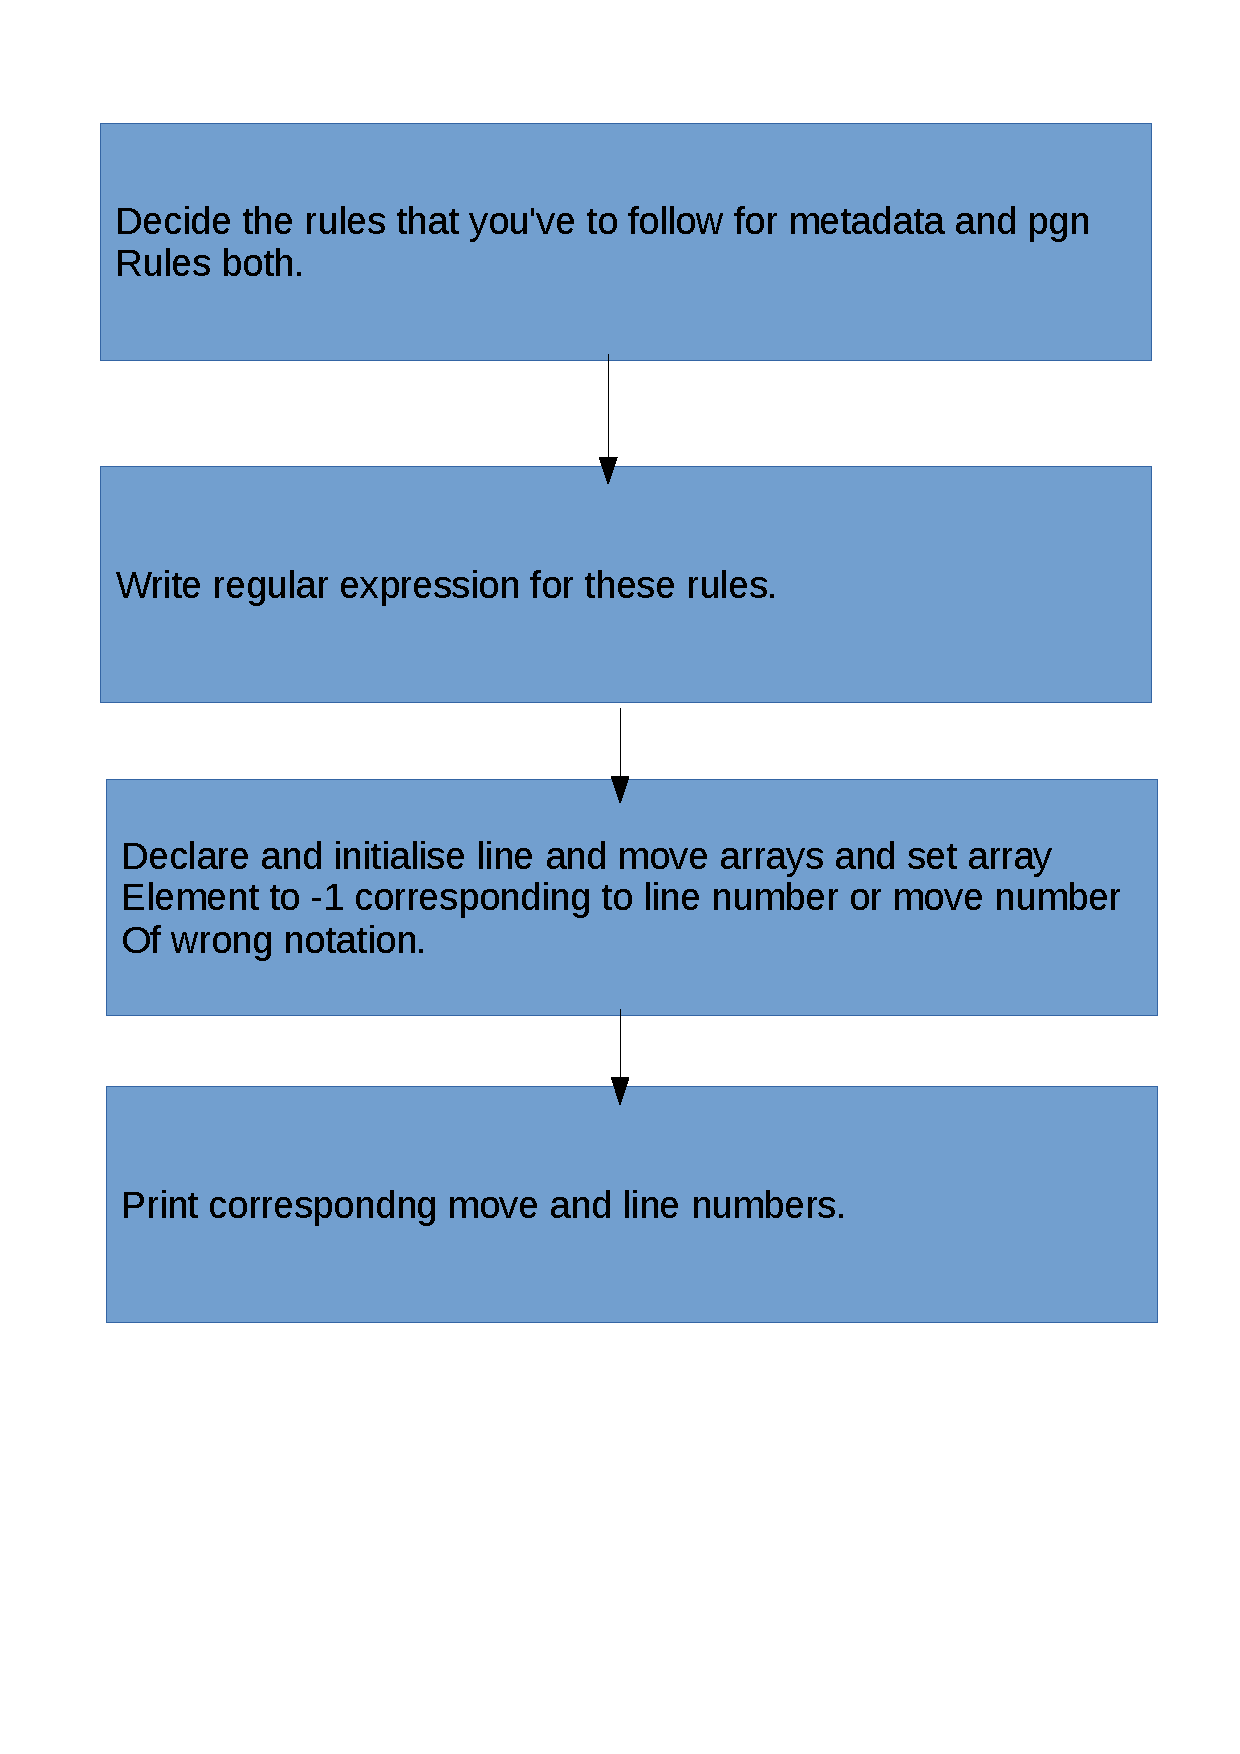
\includegraphics[scale=0.5]{images/sc1}
\caption{Structure chart for Problem 2}	
\end{figure}
\pagebreak
\section{Screenshots}
\begin{figure}[h!]
\centering
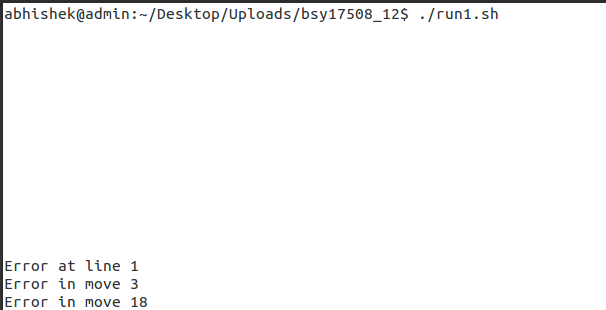
\includegraphics[scale=0.5, center]{images/screenshot1}
\caption{Screenshot for problem 1}
\end{figure}
\pagebreak
\begin{figure}[h!]
\centering
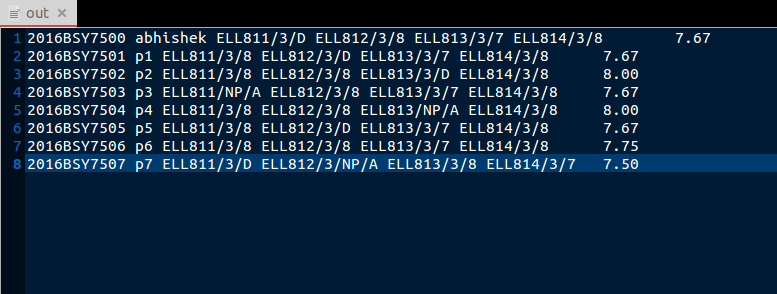
\includegraphics[scale=0.5, center]{images/screenshot2}
\caption{Screenshot for problem 2}
\end{figure}
\pagebreak
\section{Epilogue}
This week's assignment tested our scanning and parsing skills using lex and yacc implemented in linux using flex and bison. The tokens are created with the help of lex and grammar is analysed using yacc.
\bibliography{biblio} 
\bibliographystyle{ieeetr}
\nocite{*}
\end{document}